% English-only operator manual for the Ch-MBE GUI and offline RHEED labeler.
% Build from this directory with build_english_manual.ps1.
\documentclass[10pt,a4paper]{article}

\usepackage[T1]{fontenc}
\usepackage[scale=0.94]{tgheros}
\usepackage{inconsolata}
\usepackage[margin=16mm,top=18mm,bottom=17mm,headheight=14pt]{geometry}
\usepackage[table]{xcolor}
\usepackage{graphicx}
\usepackage{booktabs}
\usepackage{tabularx}
\usepackage{array}
\usepackage{enumitem}
\usepackage{microtype}
\usepackage{ragged2e}
\usepackage{fancyhdr}
\usepackage{lastpage}
\usepackage{titlesec}
\usepackage{listings}
\usepackage[most]{tcolorbox}
\usepackage{hyperref}
\usepackage{amssymb}

\ifdefined\pdfinfoomitdate
  \pdfinfoomitdate=1
\fi
\ifdefined\pdftrailerid
  \pdftrailerid{}
\fi
\ifdefined\pdfsuppressptexinfo
  \pdfsuppressptexinfo=15
\fi

\definecolor{ManualNavy}{HTML}{102A43}
\definecolor{ManualBlue}{HTML}{1565C0}
\definecolor{ManualTeal}{HTML}{00796B}
\definecolor{ManualGreen}{HTML}{2E7D32}
\definecolor{ManualAmber}{HTML}{B26A00}
\definecolor{ManualRed}{HTML}{B42318}
\definecolor{ManualLine}{HTML}{CBD5E1}
\definecolor{ManualPale}{HTML}{F4F7FA}
\definecolor{ManualBluePale}{HTML}{EAF3FF}
\definecolor{ManualGreenPale}{HTML}{EAF7EE}
\definecolor{ManualAmberPale}{HTML}{FFF6E5}
\definecolor{ManualRedPale}{HTML}{FDECEC}
\definecolor{ManualInk}{HTML}{243B53}
\definecolor{ManualMuted}{HTML}{52667A}

\hypersetup{
  colorlinks=true,
  linkcolor=ManualBlue,
  urlcolor=ManualBlue,
  pdfauthor={AI4MBE},
  pdftitle={Ch-MBE GUI and RHEED Post-processing Labeling User Manual - English Edition},
  pdfsubject={English operator guide for the Ch-MBE GUI and offline RHEED temporal labeler}
}

\renewcommand{\familydefault}{\sfdefault}
\setlength{\parindent}{0pt}
\setlength{\parskip}{4.5pt}
\setlength{\emergencystretch}{2em}
\setlist[itemize]{leftmargin=5mm,itemsep=2.5pt,topsep=2pt}
\setlist[enumerate]{leftmargin=7mm,itemsep=3pt,topsep=2pt}

\newcolumntype{Y}{>{\RaggedRight\arraybackslash}X}
\newcolumntype{L}[1]{>{\RaggedRight\arraybackslash}p{#1}}

\titleformat{\section}
  {\color{ManualNavy}\bfseries\LARGE}
  {\color{ManualBlue}\thesection}{0.65em}{}
\titlespacing*{\section}{0pt}{0pt}{5mm}
\titleformat{\subsection}
  {\color{ManualNavy}\bfseries\large}
  {}{0pt}{}
\titlespacing*{\subsection}{0pt}{4mm}{1.5mm}

\pagestyle{fancy}
\fancyhf{}
\fancyhead[L]{\small\color{ManualMuted}AI4MBE | Ch-MBE}
\fancyhead[R]{\small\color{ManualMuted}English operator manual}
\fancyfoot[L]{\small\color{ManualMuted}Manual v1.2 | 2026-08-11}
\fancyfoot[R]{\small\color{ManualMuted}Page \thepage\ of \pageref*{LastPage}}
\renewcommand{\headrulewidth}{0.4pt}
\renewcommand{\footrulewidth}{0pt}

\newtcolorbox{corebox}[1]{
  enhanced,breakable,title={#1},fonttitle=\bfseries,
  colback=ManualGreenPale,colframe=ManualGreen,coltitle=ManualGreen,
  boxrule=0.7pt,arc=2mm,left=3mm,right=3mm,top=2mm,bottom=2mm
}
\newtcolorbox{infobox}[1]{
  enhanced,breakable,title={#1},fonttitle=\bfseries,
  colback=ManualBluePale,colframe=ManualBlue,coltitle=ManualBlue,
  boxrule=0.7pt,arc=2mm,left=3mm,right=3mm,top=2mm,bottom=2mm
}
\newtcolorbox{warnbox}[1]{
  enhanced,breakable,title={#1},fonttitle=\bfseries,
  colback=ManualAmberPale,colframe=ManualAmber,coltitle=ManualAmber,
  boxrule=0.7pt,arc=2mm,left=3mm,right=3mm,top=2mm,bottom=2mm
}
\newtcolorbox{dangerbox}[1]{
  enhanced,breakable,title={#1},fonttitle=\bfseries,
  colback=ManualRedPale,colframe=ManualRed,coltitle=ManualRed,
  boxrule=0.7pt,arc=2mm,left=3mm,right=3mm,top=2mm,bottom=2mm
}

\lstdefinestyle{manualcode}{
  basicstyle=\ttfamily\small,
  backgroundcolor=\color{ManualPale},
  frame=single,
  rulecolor=\color{ManualLine},
  breaklines=true,
  columns=fullflexible,
  keepspaces=true,
  showstringspaces=false,
  aboveskip=2mm,
  belowskip=2mm,
  xleftmargin=1mm,
  framexleftmargin=1mm
}
\lstset{style=manualcode}

\newcommand{\manualsection}[2]{
  \clearpage
  \section{#2}
  \markboth{#2}{#2}
}
\newcommand{\step}[2]{
  \begin{tcolorbox}[
    enhanced,colback=white,colframe=ManualLine,boxrule=0.5pt,arc=1.5mm,
    left=2.5mm,right=2.5mm,top=1.5mm,bottom=1.5mm,before skip=1.5mm,after skip=1.5mm]
    \textcolor{ManualBlue}{\textbf{Step #1.}} #2
  \end{tcolorbox}
}
\newcommand{\checkitem}[1]{\item[$\square$] #1}
\newcommand{\manualscreenshot}[2][]{%
  \begin{center}
    \begingroup
    \setlength{\fboxsep}{1pt}%
    \color{ManualLine}\fbox{\includegraphics[#1]{#2}}%
    \endgroup
  \end{center}
}
\newcommand{\screenshotcaption}[1]{%
  \begin{center}
    {\footnotesize\color{ManualMuted}\textbf{Actual application screenshot.} #1}
  \end{center}
}

\begin{document}

% Page 1 - cover
\thispagestyle{empty}
\vspace*{4mm}
{\color{ManualNavy}\bfseries\fontsize{27}{31}\selectfont
Ch-MBE GUI and RHEED\\[1mm]
Post-processing Labeling\par}
\vspace{3mm}
{\color{ManualBlue}\fontsize{16}{20}\selectfont English Operator Manual\par}
\vspace{7mm}
\manualscreenshot[width=0.96\linewidth,height=72mm,keepaspectratio]{assets/screenshots/chmbe_growth_monitor_dummy.png}
\screenshotcaption{The current Ch-MBE Growth Monitor is running without hardware; all visible values and the RHEED frame are generated demo inputs.}
\vspace{5mm}
\begin{corebox}{Core boundary}
The post-processing labeler reads archived data only. It does not connect to or control cameras, pyrometers, power supplies, or any other instrument.
\end{corebox}
\vspace{4mm}
\rowcolors{2}{ManualPale}{white}
\begin{tabularx}{\linewidth}{L{54mm}Y}
\toprule
\textbf{Quick entry} & \textbf{Double-click} \\
\midrule
Ch-MBE live GUI & \texttt{Start Ch-MBE Growth Monitor.cmd} \\
RHEED offline labeler & \texttt{Start RHEED Post-processing Labeler.cmd} \\
Install or refresh desktop shortcuts & \texttt{Install AI4MBE Desktop Shortcuts.cmd} \\
\bottomrule
\end{tabularx}
\vfill
{\small\color{ManualMuted}
Manual v1.2 - English edition\\
Issued 2026-08-11 for the Windows Ch-MBE workstation.\\[2mm]
The screenshots show the actual applications using generated demo inputs. No experimental dataset is included.}

% Page 2 - overview
\manualsection{1}{Understand the two independent paths}

The live GUI performs acquisition and display. The offline labeler works only on completed archived sessions. Never interpret an offline result as a real-time control instruction.

\begin{center}
\begin{minipage}[t]{0.485\linewidth}
  \centering
  \begingroup\setlength{\fboxsep}{1pt}\color{ManualLine}
  \fbox{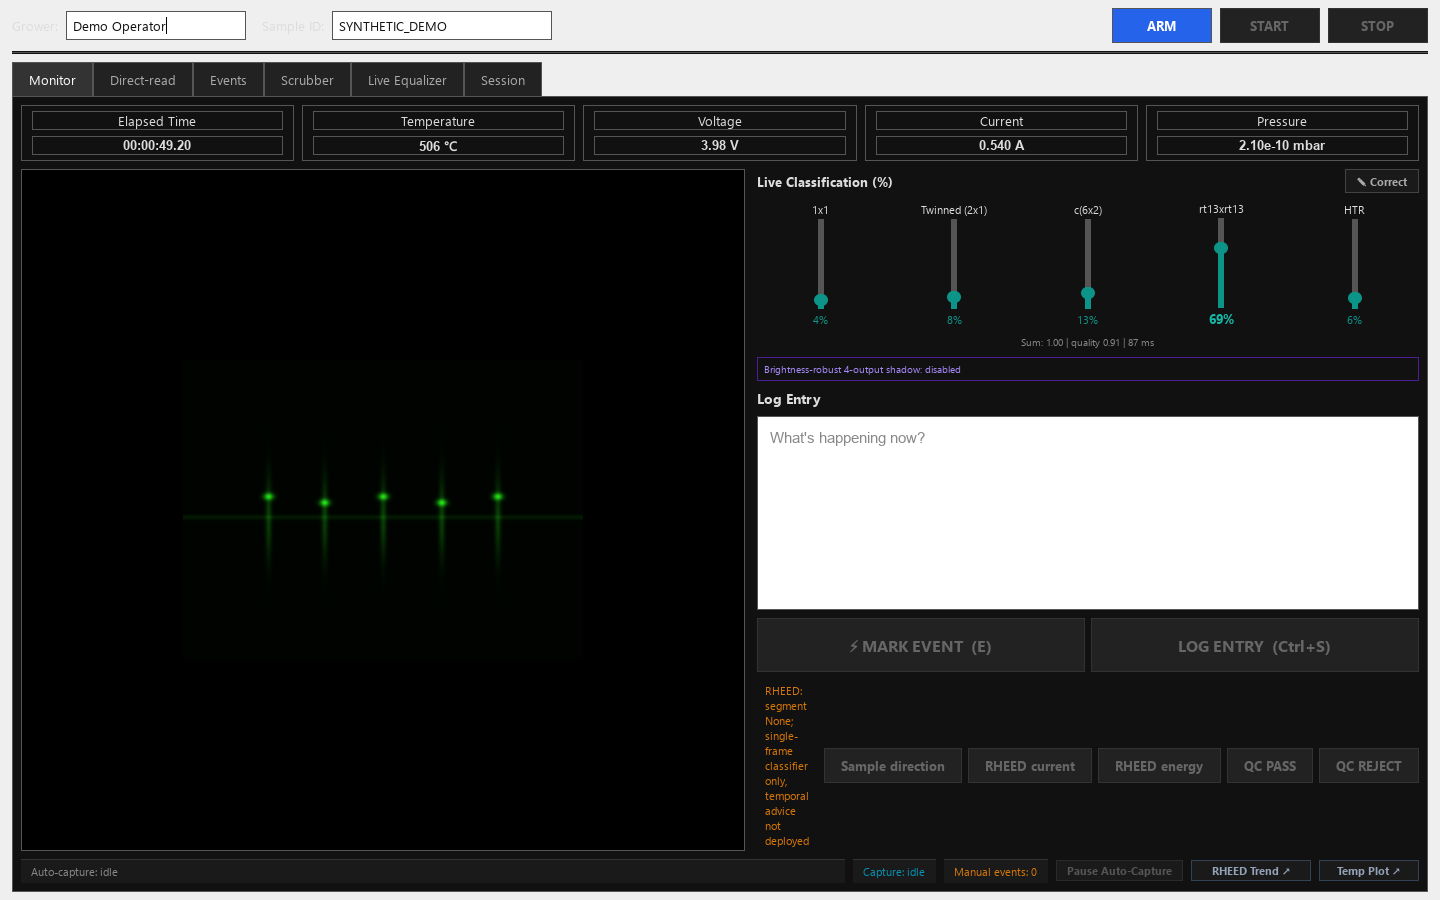
\includegraphics[width=0.96\linewidth]{assets/screenshots/chmbe_growth_monitor_dummy.png}}
  \endgroup\\[-1mm]
  {\footnotesize\textbf{1. Live acquisition}\par}
  {\scriptsize\color{ManualMuted}Growth Monitor writes the archived session.\par}
\end{minipage}\hfill
\begin{minipage}[t]{0.485\linewidth}
  \centering
  \begingroup\setlength{\fboxsep}{1pt}\color{ManualLine}
  \fbox{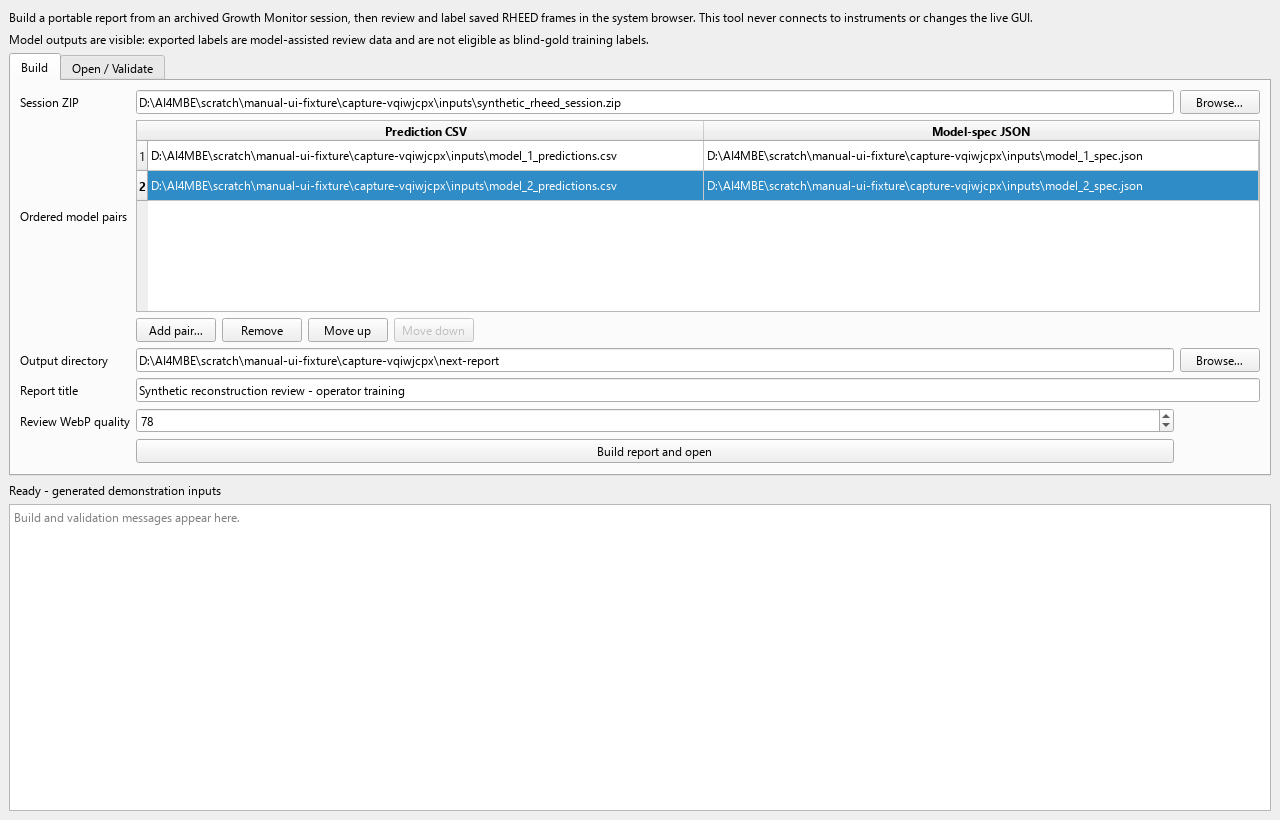
\includegraphics[width=0.96\linewidth]{assets/screenshots/rheed_labeler_build.png}}
  \endgroup\\[-1mm]
  {\footnotesize\textbf{2. Offline build and validation}\par}
  {\scriptsize\color{ManualMuted}The labeler combines the ZIP with predictions and model specifications.\par}
\end{minipage}
\end{center}
\begin{corebox}{The boundary between the applications}
The live GUI creates session records. The labeler reads those records later, produces a browser report, and exports validated JSON. It never sends commands back to the instruments.
\end{corebox}

\subsection{What this manual covers}
\rowcolors{2}{ManualPale}{white}
\begin{tabularx}{\linewidth}{L{16mm}L{72mm}Y}
\toprule
\textbf{Page} & \textbf{Topic} & \textbf{Outcome} \\
\midrule
3 & Shortcuts and live GUI startup & Confirm the correct chamber and a clean exit \\
4 & Labeler desktop application & Select inputs, build, open, and validate \\
5-6 & Inputs and safe report build & Produce a complete local report directory \\
7-8 & Segment labeling and display controls & Create traceable labels on actual saved frames \\
9 & Export, import, and validation & Produce canonical JSON and validate fail-closed \\
10-12 & Safety, troubleshooting, and version checks & Handoff and reproduce the work safely \\
\bottomrule
\end{tabularx}

\begin{warnbox}{Keep the concepts separate}
Surface-reconstruction labels, acquisition-quality QC, and FeSe film quality are three different concepts. The current classifier concerns the bare STO surface before growth.
\end{warnbox}

\subsection{Operating principle}
\begin{itemize}
  \item The GUI reads live instrument sources and writes session records under the operator's control.
  \item Post-processing combines an archived session with one or more already-generated prediction tables.
  \item Human labels are stored as frame-bound temporal segments with provenance.
  \item Model outputs remain visible, so these annotations are assisted review, not blind-gold labels.
\end{itemize}

% Page 3 - live GUI
\manualsection{2}{Install shortcuts and start the Ch-MBE GUI}

\subsection{First setup or after moving the checkout}
\step{1}{From the GUI repository root, double-click \texttt{Install AI4MBE Desktop Shortcuts.cmd}.}
\step{2}{Confirm that the desktop contains refreshed shortcuts named \textbf{Ch-MBE Growth Monitor} and \textbf{RHEED Post-processing Labeler}.}
\step{3}{If Windows displays an unexpected security warning, do not bypass it. Stop and ask the maintainer to verify the file source and commit.}

\subsection{Start each experiment}
\step{1}{Double-click \texttt{Start Ch-MBE Growth Monitor.cmd} or its desktop shortcut. Do not use an O-MBE launcher.}
\step{2}{Wait for the main window and confirm the title \textbf{Chalcogenide MBE Growth Monitor}. Then inspect each device status.}
\step{3}{ARM or start a session only when the operator is ready under the experiment SOP. Double-click startup does not authorize setpoint changes.}
\step{4}{At the end, close through the GUI normally and wait for the window to disappear. Do not force-kill Python while logs are being written.}

\manualscreenshot[width=0.78\linewidth,height=58mm,keepaspectratio]{assets/screenshots/chmbe_growth_monitor_session.png}
\screenshotcaption{The current Session tab in a hardware-free demo. Confirm the chamber and every selected interface before ARM.}

The launcher forces the Ch-MBE chamber configuration and refuses a second live-GUI process through a Windows single-instance mutex.

Before ARM, confirm the Ch-MBE chamber, an advancing RHEED frame sequence, a valid temperature state, and the intended log directory.

\begin{infobox}{Expected environment behavior}
Launcher logs are stored below \texttt{\%LOCALAPPDATA\%\textbackslash AI4MBE\textbackslash LauncherLogs}. They record the resolved Python interpreter, repository path, branch, commit, chamber, and optional driver status. Missing \texttt{pyads}, \texttt{serial}, or \texttt{windows\_capture} produces a visible warning without hiding the GUI; do not ARM a production mode that needs the missing driver. Do not assume a fixed drive letter or create global environment variables ad hoc.
\end{infobox}

% Page 4 - labeler UI
\manualsection{3}{Open the RHEED post-processing labeler}

\step{1}{Double-click \texttt{Start RHEED Post-processing Labeler.cmd} or its desktop shortcut.}
\step{2}{Confirm that the application has the \textbf{Build} and \textbf{Open / Validate} tabs, plus \textbf{Build report and open}, \textbf{Open report}, \textbf{Validate annotations}, and \textbf{Open English PDF manual}. It must not start Growth Monitor or contact instruments.}

\manualscreenshot[width=0.90\linewidth,height=92mm,keepaspectratio]{assets/screenshots/rheed_labeler_build.png}
\screenshotcaption{The current desktop labeler Build tab populated with a generated local fixture. The application is offline and no instrument process is running.}

\rowcolors{2}{ManualPale}{white}
\begin{tabularx}{\linewidth}{L{42mm}Y}
\toprule
\textbf{Area} & \textbf{Purpose} \\
\midrule
Session ZIP & Select one archived Growth Monitor session \\
Model inputs & Pair one prediction CSV with its model-spec JSON on each row \\
Output directory & Select a new or empty directory, preferably outside Git \\
Message log & Preserve complete build and validation messages \\
Open report button & Open a previously generated \texttt{interactive\_report.html} \\
Validate annotations & Check exported JSON against the exact report provenance \\
\bottomrule
\end{tabularx}

\begin{corebox}{Offline by design}
This application can run on a computer without instrument software when the archived inputs are complete and the Python environment is valid. Report construction and validation run in an isolated child process so the desktop application remains responsive.
\end{corebox}

% Page 5 - inputs
\manualsection{4}{Prepare inputs and verify provenance}

\subsection{Session archive}
The ZIP archive must contain exactly one member ending in \texttt{session\_metadata.json}, exactly one member ending in \texttt{heartbeat\_log.csv}, and every sibling \texttt{frames/} image referenced by the heartbeat rows. Saved-frame elapsed time, heartbeat index, capture sequence, and timezone-aware capture UTC must each increase strictly; gaps are allowed. Do not extract and rename frames manually.

\begin{lstlisting}
growth_session.zip
  session_metadata.json
  heartbeat_log.csv
  frames/
    heartbeat_000001_....bmp
    heartbeat_000002_....bmp
\end{lstlisting}

\subsection{Prediction tables and model specifications are positional pairs}
\rowcolors{2}{ManualPale}{white}
\begin{tabularx}{\linewidth}{L{31mm}L{82mm}Y}
\toprule
\textbf{File} & \textbf{Required content} & \textbf{Check} \\
\midrule
Prediction CSV & frame index, heartbeat index, elapsed time, capture UTC, capture sequence, frame name, frame SHA-256, and score columns & Rows match the saved-frame order exactly \\
Model-spec JSON & schema version 1, non-empty key and title, at least two unique classes, and equally sized unique probability columns & Class order matches the score columns; status and provenance are optional \\
Session ZIP & metadata, heartbeat log, and frames & Every referenced frame exists in the archive \\
\bottomrule
\end{tabularx}

Prediction \texttt{frame\_index} may begin at 0 or 1, but it must then remain contiguous. Heartbeat indices, capture sequences, and elapsed times may contain gaps. The tool follows actual saved frames and recorded times; it never assumes exact 1 Hz sampling.

\begin{dangerbox}{Fail closed}
Any mismatch in row count, order, time, sequence, filename, or SHA-256 stops the build. Do not edit the inputs to bypass an error.
\end{dangerbox}

\subsection{Recommended local layout}
\begin{lstlisting}
<local-data-root>\2026-08-11_anneal\
  source\growth_session.zip
  predictions\model_A.csv
  specs\model_A.json
  output\
  exports\
\end{lstlisting}

% Page 6 - build
\manualsection{5}{Build and open a report safely}

\step{1}{Choose the preserved archive copy in Session ZIP.}
\step{2}{Add one Prediction CSV and Model-spec JSON row for every model to display. Pairing is positional, so preserve row order.}
\step{3}{Choose a new or empty directory outside the repository. The desktop labeler will not overwrite a non-empty directory.}
\step{4}{Enter a report title. Review quality changes only the lossy review images; it never changes archived pixels or model predictions. The default value of 78 is suitable for routine use.}
\step{5}{Click \textbf{Build report and open}. Wait for success and for \texttt{interactive\_report.html} to open automatically.}

\subsection{PowerShell fallback}
\begin{lstlisting}
Set-Location '<GUI repository>'
conda activate ai4mbe-gui
python -m tools.rheed_postprocessing_labeling build `
  --session '<local-data-root>\growth_session.zip' `
  --predictions '<local-data-root>\predictions.csv' `
  --model-spec '<local-data-root>\model_spec.json' `
  --output-dir '<local-data-root>\labeling-output'
\end{lstlisting}

\subsection{Copy the entire report directory}
The report consists of \texttt{interactive\_report.html}, \texttt{images/}, \texttt{vendor/}, and \texttt{run\_manifest.json}. Copy the entire directory during handoff. Preserve the original prediction CSV and model-spec JSON separately outside the report directory.

\begin{warnbox}{Advanced CLI overwrite boundary}
The desktop application always refuses a non-empty output directory. CLI \texttt{-{}-overwrite} may replace only a recognized, unmodified tool output. It validates the new inputs and stages a complete replacement first. If the old report changes during the build, replacement stops and the original content is restored. Filesystem roots, repository paths, the current directory, and directories containing inputs are always rejected.
\end{warnbox}

% Page 7 - annotation
\manualsection{6}{Label temporal segments like an editing timeline}

\manualscreenshot[width=0.94\linewidth,height=104mm,keepaspectratio]{assets/screenshots/rheed_timeline_editor.png}
\screenshotcaption{The current English browser editor with generated RHEED frames, synthetic model curves, saved human segments, and a synchronized playhead.}

\step{1}{Move the Frame playhead or click a model plot to locate the first saved frame of a segment. Click \textbf{Mark In}.}
\step{2}{Move to the final saved frame of the segment and click \textbf{Mark Out}. The Out marker is inclusive.}
\step{3}{Choose a reconstruction label, enter the labeler name, add notes when useful, and click \textbf{Add segment}.}
\step{4}{Select a saved segment to edit it. Update preserves its annotation ID. Adjacent segments are allowed; overlapping segments are rejected.}

The displayed and exported saved-frame ordinal is 1-based. Every endpoint also records heartbeat index, capture sequence, UTC, and frame SHA-256. This preserves traceability even when the sampling interval or sequence contains gaps.

\begin{infobox}{Frame-bound interval semantics}
Labels cover the saved frames from In through Out, inclusive. They do not claim that unsaved camera frames or every capture-sequence number in between was reviewed.
\end{infobox}

% Page 8 - review controls
\manualsection{7}{Review, display controls, and drafts}

\subsection{All time indicators remain synchronized}
\rowcolors{2}{ManualPale}{white}
\begin{tabularx}{\linewidth}{L{38mm}L{68mm}Y}
\toprule
\textbf{Action} & \textbf{Must update together} & \textbf{Must not change} \\
\midrule
Move the main timeline & Current RHEED image, model guides, enlarged-view timeline & Archive and prediction values \\
Click a model curve & Main playhead, image, and metadata & Saved segments \\
Adjust brightness or contrast & On-screen appearance & Pixels, SHA-256, and model outputs \\
Enlarge the image & Zoom view and its adjustable timeline & Source image and segment boundaries \\
\bottomrule
\end{tabularx}

\manualscreenshot[width=0.76\linewidth,height=70mm,keepaspectratio]{assets/screenshots/rheed_timeline_zoom.png}
\screenshotcaption{The actual enlarged-frame dialog. Its timeline changes the selected frame while preserving zoom, pan, and display adjustments.}

\subsection{Drafts and editing}
\begin{itemize}
  \item The browser stores a draft scoped by both dataset ID and model-context fingerprint in localStorage. This is not a durable backup.
  \item Export JSON frequently, especially during long reviews and before changing computers, browsers, or cache settings.
  \item Delete selected requires confirmation. Undo restores only the most recent annotation mutation.
  \item Import JSON validates before replacement. On failure, the current segment set remains unchanged.
\end{itemize}

\subsection{Interpretation}
Labels describe the dominant surface-reconstruction category seen by the reviewer during the interval. The displayed \textbf{Uncertain} label exports as \texttt{unknown}; \textbf{1x1 / none-weak} exports as \texttt{none\_weak}. Never overwrite a human selection with model argmax, and never interpret \texttt{unknown} as acquisition-quality rejection.

\begin{infobox}{Display adjustment is not data modification}
Brightness, contrast, zoom, and image enlargement aid inspection only. Brightness and contrast are stored with each segment; zoom is not exported. The report never rewrites archived images or model outputs.
\end{infobox}

Use a four-pass review rhythm: survey the full run, confirm every In and Out
frame, inspect gaps and uncertain labels, then export and validate the canonical
JSON.

% Page 9 - export
\manualsection{8}{Export, import, and fail-closed validation}

\subsection{JSON is the canonical artifact}
Use Export JSON to resume work, validate provenance, and support downstream processing. Export CSV is useful for meetings and tabular analysis, but it does not replace the complete nested provenance in JSON.

\rowcolors{2}{ManualPale}{white}
\begin{tabularx}{\linewidth}{L{66mm}Y}
\toprule
\textbf{Binding} & \textbf{Purpose} \\
\midrule
\texttt{dataset\_id} and source archive SHA-256 & Bind the source session \\
Ordered-frame fingerprint & Bind frame order and per-frame SHA-256 \\
\texttt{model\_context\_fingerprint} & Bind the visible predictions and model specifications \\
Endpoint provenance & Bind saved-frame ordinal, heartbeat, UTC, sequence, and SHA-256 \\
\texttt{model\_outputs\_visible=true} & Disclose that the models were visible \\
\texttt{eligible\_for\_gold=false} & Prevent blind-gold misuse \\
\bottomrule
\end{tabularx}

\subsection{Validate in the desktop application}
\step{1}{Select the original \texttt{interactive\_report.html}.}
\step{2}{Select the exported annotation JSON.}
\step{3}{Click \textbf{Validate annotations}. Continue only when the application says \textbf{Annotation JSON is valid for this report}.}

\subsection{PowerShell validation}
\begin{lstlisting}
python -m tools.rheed_postprocessing_labeling validate `
  --report '<local-data-root>\labeling-output\interactive_report.html' `
  --annotations '<local-data-root>\exports\segment_annotations.json'
\end{lstlisting}

\begin{dangerbox}{Never bypass a validation failure}
A wrong run, changed model context, altered endpoint, overlapping segment, invalid label, or gold-data claim causes validation to fail. Return to the correct report and original export and investigate the exact message.
\end{dangerbox}

Browser Import performs immediate client-side provenance checks before replacing the current draft. Desktop \textbf{Validate annotations} is the authoritative full fail-closed validation.

% Page 10 - safety
\manualsection{9}{Data safety and scientific boundaries}

\subsection{What belongs in Git}
\rowcolors{2}{ManualPale}{white}
\begin{tabularx}{\linewidth}{Y Y}
\toprule
\textbf{May be tracked} & \textbf{Keep out by default} \\
\midrule
Tool code, templates, tests, and documentation & Real session ZIP files, raw RHEED images, and sensor logs \\
Example model specifications & Real predictions, generated reports, and annotation JSON or CSV \\
Sanitized documentation screenshots made with generated demo inputs & Checkpoints, unpublished results, and experiment-specific screenshots \\
\bottomrule
\end{tabularx}

\subsection{Safe handling sequence}
\step{1}{Keep the source session ZIP read-only or preserve an immutable copy, and record its SHA-256.}
\step{2}{Create a dedicated working directory outside the repository. Keep reports, exports, and screenshots there.}
\step{3}{For handoff, copy the complete report directory and canonical JSON. Separately preserve the original prediction CSV, model-spec JSON, and SHA manifest. Never send only the HTML.}
\step{4}{Run statistics or training-data preparation only after validation, and preserve the original export unchanged.}

\begin{dangerbox}{Model-assisted review, not blind-gold}
Model plots and lossy review images are visible during labeling. These annotations are eligible only as model-assisted review. Formal blind-gold labels require a separate workflow that hides model and Equalizer outputs and preserves the required audit evidence.
\end{dangerbox}

\begin{warnbox}{Do not over-interpret the output}
The current classification target is bare STO surface reconstruction before growth. Do not interpret a reconstruction label as FeSe film quality. Do not equate reconstruction \texttt{unknown} with acquisition-quality \texttt{QC\_REJECT}.
\end{warnbox}

% Page 11 - troubleshooting
\manualsection{10}{Troubleshooting}

First preserve the exact error text, occurrence time, branch, commit, and selected paths. Do not begin by deleting environments, changing global variables, or force-resetting Git. A live-driver warning is fail-visible behavior, not a prompt for ad hoc dependency installation.

\small
\rowcolors{2}{ManualPale}{white}
\begin{tabularx}{\linewidth}{L{37mm}L{50mm}Y}
\toprule
\textbf{Symptom} & \textbf{Likely cause} & \textbf{Safe action} \\
\midrule
Desktop shortcut is absent or opens an old checkout & Installer was not run after the checkout moved & Run the shortcut installer from the current repository root \\
Growth Monitor shows the wrong chamber & Wrong launcher was used & Close normally and use only the Ch-MBE launcher \\
Launcher window closes immediately & Environment or dependency failure & Read the newest launcher log; if needed, run the same CMD from PowerShell \\
Temperature or RHEED has no valid reading & Interface, vendor window, or selected mode issue & Record connected, error, and mode; do not guess global settings \\
Labeler rejects Build & Missing input, mismatched pair, or non-empty output & Check the session, each positional pair, and a new output directory \\
Provenance mismatch & Predictions do not belong to the ZIP or rows changed & Find the matching predictions and spec; do not edit the CSV \\
HTML has no images or curves & Only the HTML was copied or assets are missing & Restore the complete report directory and relative paths \\
Draft disappeared & Browser, computer, or localStorage changed & Import the latest JSON and export more frequently \\
Import or validation fails & Run, context, endpoint, overlap, or label mismatch & Use the original report and JSON; read the fail-closed message \\
\bottomrule
\end{tabularx}
\normalsize

\subsection{Minimum evidence for the maintainer}
\begin{itemize}
  \item Full error text and occurrence time. Do not report only that it does not work.
  \item Output of \texttt{git status -{}-short -{}-branch} and \texttt{git rev-parse HEAD}.
  \item Launcher name, environment path, input filenames, and output directory. Keep sensitive data out of public channels.
  \item For labeling issues, report-manifest and annotation-JSON SHA values. Raw images are not initially required.
\end{itemize}

% Page 12 - checklist
\manualsection{11}{Version verification and quick checklist}

\subsection{Record versions before acquisition or labeling}
\begin{lstlisting}
Set-Location '<GUI repository>'
git status --short --branch
git rev-parse HEAD
conda env list
conda activate ai4mbe-gui
python --version
python -m tools.rheed_postprocessing_labeling --help
\end{lstlisting}

Use the resolved Python interpreter and repository path recorded by the launcher. Read \texttt{AI4MBE\_GUI\_PYTHON} only when it is already configured on that workstation; do not create it ad hoc. If the branch or commit differs from the team-specified version, or Git reports unknown modifications, stop and verify.

\subsection{Integrity hashes}
\begin{lstlisting}
Get-FileHash '<local-data-root>\growth_session.zip' -Algorithm SHA256
Get-FileHash '<local-data-root>\exports\segment_annotations.json' -Algorithm SHA256
Get-FileHash '.\docs\RHEED_GUI_Postprocessing_Labeling_User_Manual_EN.pdf' -Algorithm SHA256
\end{lstlisting}

\subsection{Quick checklist}
\begin{itemize}[leftmargin=7mm,itemsep=1.7pt]
  \checkitem{Use the Ch-MBE launcher and confirm the chamber identity.}
  \checkitem{Confirm live status, frame sequence, temperature, and logging behavior under the experiment SOP.}
  \checkitem{Preserve a read-only source ZIP and its SHA-256.}
  \checkitem{Open the offline labeler with the dedicated launcher.}
  \checkitem{Pair every prediction CSV with the correct model-spec JSON.}
  \checkitem{Use a new or empty output directory outside Git.}
  \checkitem{Review boundaries frame by frame; allow no overlaps.}
  \checkitem{Export JSON and validate it against the original report.}
  \checkitem{Record branch, commit, environment, manifest, and export hashes.}
  \checkitem{Handoff the complete report and declare model-assisted, not blind-gold.}
\end{itemize}

\begin{dangerbox}{Stop condition}
Stop and contact the maintainer when instrument state, stale data, version identity, provenance, or validation cannot be explained.
\end{dangerbox}

\vfill
\hrule
\vspace{2mm}
{\small\color{ManualMuted}Application screenshots were captured from the actual software using generated demo inputs; they contain no experimental data.}

\end{document}
